\documentclass[12pt,twocolumn,letterpaper]{article}

\usepackage{statcourse}
\usepackage{times}
\usepackage{epsfig}
\usepackage{graphicx}
\usepackage{amsmath}
\usepackage{amssymb}

% Include other packages here, before hyperref.

% If you comment hyperref and then uncomment it, you should delete
% egpaper.aux before re-running latex.  (Or just hit 'q' on the first latex
% run, let it finish, and you should be clear).
\usepackage[breaklinks=true,bookmarks=false]{hyperref}


\statcoursefinalcopy


\setcounter{page}{1}
\begin{document}


%%%%%%%%%%%%%%%%%%%%%%%%%%%%%%%%%%%%%%%%%%%%%%%%%%%%%%%%%%%%%%%
% DO NOT EDIT ANYTHING ABOVE THIS LINE
% EXCEPT IF YOU LIKE TO USE ADDITIONAL PACKAGES
%%%%%%%%%%%%%%%%%%%%%%%%%%%%%%%%%%%%%%%%%%%%%%%%%%%%%%%%%%%%%%%



%%%%%%%%% TITLE
\title{What are you drawing? Classifying Goodle Quick Draw Doodles}

\author{First Author\\
{\tt\small firstauthor@wisc.edu}
\and
Second Author\\
{\tt\small secondauthor@wisc.edu}
\and
Third Author\\
{\tt\small thirdauthor@wisc.edu}
}

\maketitle
%\thispagestyle{empty}



% MAIN ARTICLE GOES BELOW
%%%%%%%%%%%%%%%%%%%%%%%%%%%%%%%%%%%%%%%%%%%%%%%%%%%%%%%%%%%%%%%


%%%%%%%%% ABSTRACT
\begin{abstract}
Image recognition, especially from scratchy and noisy data, plays a significant role in machine learning. In our project we want to classify the hand-drawn doodles, with 345 categories in total, from Google Quick Draw. We construct different algorithms such as kNN, Logistic Regression, Support Vector Machine, and Convolutional Neural Network, and they each obtains an accuracy of {}. We also experimented different dimensionality reduction methods for kNN and Logistic Regression. By comparing model performance, we can gain an insight on which classifier is the most suitable for classifying doodles with a lot of categories.
\end{abstract}

% 要用现在时

%%%%%%%%% BODY TEXT
\section{Introduction}

Quick, Draw!\footnote{https://quickdraw.withgoogle.com/} is an online game released by Google on November, 2016 where the user is prompted with a specific requirement to draw a picture in 20 seconds and the algorithm will make a prediction based on the drawing. Millions of images were collected by Google through this game, and they were utilized to make better and quicker predictions. Figure \ref{fig:quickdraw} showed an example of such images\footnote{https://github.com/googlecreativelab/quickdraw-dataset}. Such large-scale data set leaves many to the imagination of machine learning enthusiasts and encourages the rises of creative projects. For example, Quartz has explored the drawing habits like stroke order grouped by different countries and found clear associations between the drawing and their language styles \cite{quartzcircle}; others tried several different prediction models evaluated by prediction accuracy \cite{github}.

More than simply classifying doodles, such algorithms could have educational applications for language-learning toddlers as well. They can draw what they see, and learn how to spell or say it, which could accelerate the language learning process. Moreover, since doodles are somewhat sketchy, by constructing algorithms that can make accurate predictions based on sketchy images, the uses of the algorithms could be extended to convert handwritten text to computer, eliminating the need to type all the words.

In our project, rather than building seperate algorithms for each category or subset of categories, we combined all categories together as our data set. Therefore, since our data set has 345 categories in total, the prediction accuracy is not very high, but is still higher than what we expected. We apply several algorithms such as kNN, Logistic Regression, SVM, and Convolutional Neural Network, and adopt different variations of dimensionality reduction methods.

\begin{figure}[h]
\begin{center}
   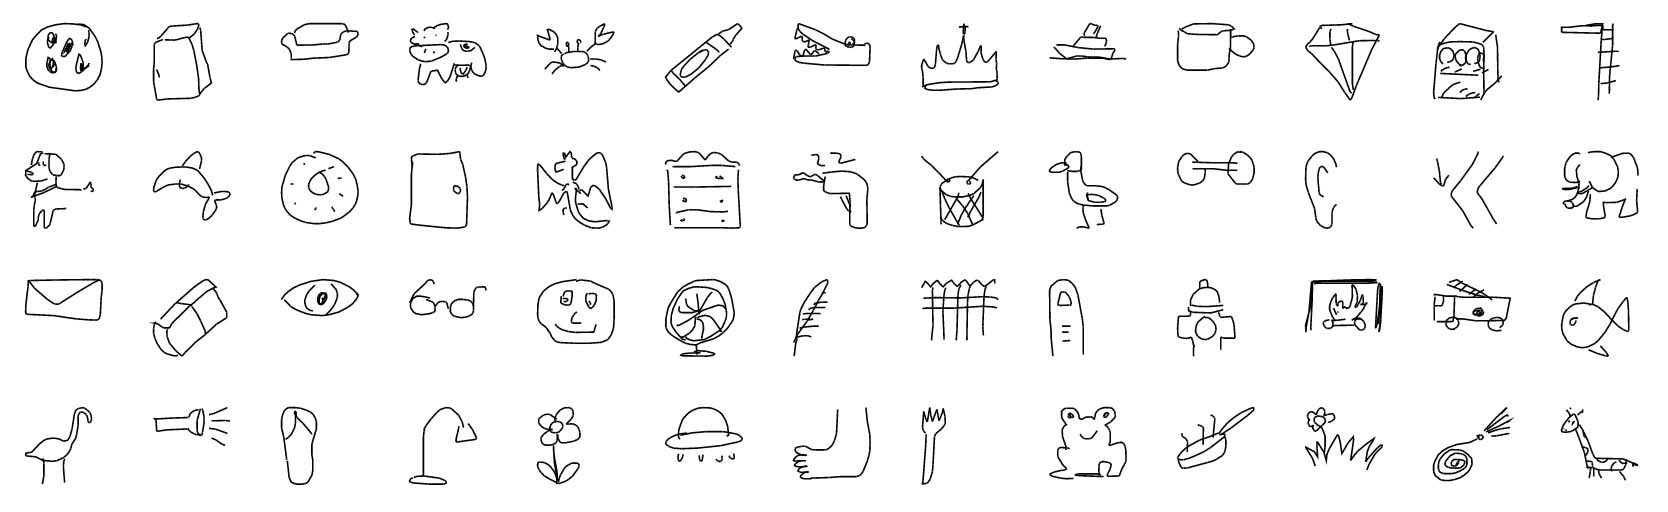
\includegraphics[width=0.8\linewidth]{figures/quickdraw_image.jpg}
\end{center}
   \caption{Example of quick draw imgaes}
\label{fig:quickdraw}
\end{figure}


\begin{figure}[h]
\begin{center}
   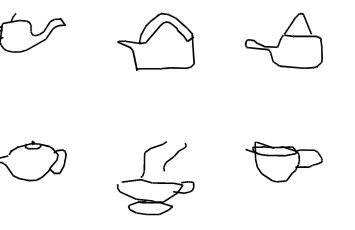
\includegraphics[width=0.8\linewidth]{figures/teapot.png}
\end{center}
   \caption{Example drawings of teapot}
\label{fig:teapot}
\end{figure}

\section{Related Work}

Related work should be discussed here. This is an example of a citation. To format the citations properly, put the
corresponding references into the bibliography.bib file. You can obtain
BibTeX-formatted references for the "bib" file from Google Scholar 
(\url{https://scholar.google.com}), for example, by clicking on the 
double-quote character under a citation and then selecting \mbox{"BibTeX"} as
shown in Figure \ref{fig:google-scholar-1col} and 
Figure \ref{fig:google-scholar-2col}.


Table \ref{tab:some-table} shows an example for formatting a table.

\begin{table}
\begin{center}
\begin{tabular}{|l|c|}
\hline
Method & Accuracy \\
\hline\hline
Method 1 & $70 \pm 3$ \% \\
 Method 2 & $76 \pm 3$ \% \\
\hline
\end{tabular}
\end{center}
\label{tab:some-table}
\caption{This is an example of a table.}
\end{table}


\section{Proposed Method}

The data we have in hand is in the general form of typical image data, with 784 dimensions, each representing a pixel of the image. When firstly look at out data, we find the data has a bunch of uninformative features, i.e. the dataset have a lot of features with value zero for all images. Therefore, we decided to apply dimensionality reduction methods to get rid of such unuseful features and to improve computational efficiency. 

We start building the classifier with kNN, which is a lazy algorithm that does not learn from the data but simply memorize. We then fit the data into penalized multinomial logistic regression with cross-validation. Then we use Support Vector Machine and Convolutional Neural Network to classify the doodles. We define the accuracy score by the proportion of the number of doodles correctly classified.

$$ACC = \frac{\# Correctly Classified}{\# Doodles}$$

We randomly split our data into 80\% training and 20\% testing.

\subsection{k-Nearest Neighbors}

The first method that comes in mind when doing classification tasks is the k-Nearest Neighbors algorithm. It is a lazy algorithm that simply memorize the data. kNN algorithms takes two parameters: k, the number of neigherbors to be considered, and p, the parameter for the Minkowski distance function. Minkowski distance is defined as
$$D(\mathbf{X}, \mathbf{Y}) = (\sum_{i = 1}^{n} (\lvert x_i - y_i \rvert)^p)^\frac{1}{p}}$$
And this distance corresponds to the Manhattan Distance when p = 1, and Euclidean Distance when p = 2.
 
When classying a data point, kNN calculates the k nearest neighbors by the Minkowski distance defined by p, get their labels, and then determine the label of the new data through majority (or plurality) voting. To obtain the optimal k, we conduct 5-fold cross validation on the training set. To wit, the training set is split into 5 portions, and the algorithm is fit five times. Each time the kNN use 4 portions as training and the reamining one as validation. The final accuracy is obtained by averaging the performance of the 5 validation sets in each fitting. In addition, since kNN can be susceptible to the curse of dimensionality, we apply two dimensionality reduction methods: Principal Component Analysis and Autoeocoder.  %可以加一个5-foldcv的图%  , %介绍一下PCA 和 AE%
The number of optimal components is also obtained through cross-validation. While the num_hidden layer in Autoencoder is the same as PCA n_components. 

\subsection{Multinomial Logistic Regression}

We then fit the data into multinomial logistic regression with L1 penalty (LASSO). %加一个feature_selection里那个L1的图%
Multinomial logistic regression returns the probabity of the label equals to k with the following equation
$$\mathbf{Pr}(Y^{[i]} = k) = \frac{e^{\beta_k \mathbf{X}^{[i]}}}{\sum_{i = 1}^{K} e^{\beta_i} \mathbf{X}^{[i]}}$$

To prevent this model from overfitting the data, we apply L1 penalty to the model, with coefficient \lambda obtained through 5-fold cross validation. We also use the two dimensionality reduction methods as mentioned above to accelerate computational time. 

\subsection{Support Vector Machine}

\subsection{Convolutional Neural Network}

Describe the method(s) you are proposing, developing, or using. I.e., details
of the algorithms may be included here. 

\section{Experiments}


\subsection{Dataset}

The original data set we have consists of 345 Numpy Bitmap files from Google, each npy consists of thousands of gray scale images for each category. Google has already preprocessed the data in npy files by only keeping image data and centering the image with 28 * 28 pixels. Because it is not practical to run the whole data set on our computer, we decide to take a random sample of 1000 images from each category, and combined them to one single npy file, which has 345,000 images in total. In fitting the models, we split our data set as 80\% for training and 20\% for testing using $train_test_split$ in Sci-Kit Learn stratified on labels. Each image is represented as having 784 dimensions, with values representing the intensity of each pixel, ranging from 0 - 255. We apply max-min normalization to the image data, and the range thus becomes 0 - 1. In addition, the label is represented as 0 - 344 for each category, rather than the eaxt text label. Global random seed is set at 123.

\subsection{Dimensionality Reduction}

\paragraph{PCA}
Since image is centered, we find that there are a lot of features that are all zeroes for all images, thus making them unimformative in model prediction. Therefore, we decide to use Principal Component Analysis to get rid of uninformative features and reduce dimensions. We firstly graphed the explained variance of the feature %加pca那个图%,
we find that 256 features already explain 100\% of the variance in the data, and that there does not seem to be a much difference between 100, 200, and 256. Thus we apply cross-validation to find the optiomal number of components for kNN and Logistic Regression, and 100 components are suggested for both methods. 

\paragraph{Autoencoder}

%parameter settings, details, graph前后对比, num_hidden = 100 because pca = 100 to make consistent. %

\subsection{k-Nearest Neighbors}

To obtain the optimal choice of k and n_components, we use the GridSearchCV function with 5-fold cross validation. We make a pipeline to determine the combination. For PCA the number of components to be chosen from are [100, 200, 256], and for k the range is [5,100] with step = 5. Since our data set is too large and GridSearchCV failed to return the result even after one and a half days, we decided to run it on a smaller subset with 200 images for each category. This greatly enhanced the computational time. We also fit the kNN model on the original dataset with 784 dimensions to compare the results.

\subsection{Multinomial Logistic Regression}

\subsection{Support Vector Machine}

\subsection{Convolutional Neural Network}



\section{Results and Discussion}




\section{Conclusions}

Describe your conclusions here. If there are any future directions, you can
describe them here, or you can create a new section for future directions.

\section{Acknowledgements}

%include ae and cnn code source

List acknowledgements if any. For example, if someone provided you a dataset, or
you used someone else's resources, this is a good place to acknowledge
the help or support you received.

\section{Contributions}

Describe the contributions of each team member who worked on this project.


{\small
\bibliographystyle{ieee}
\bibliography{bibliography}
}

\end{document}
